\documentclass[spanish]{beamer}
\usepackage{graphicx}

% Tema de la presentación
\usetheme{metropolis}

% Información del documento
\title{Detección de defectos en objetos en movimiento mediante Redes Neuronales Convolucionales con optimizaciones específicas para hardware NVIDIA}

\date{11 de julio de 2025}
\author{Alumno: Haro Armero, Abel \\ Tutor: Flich Cardo, José \\ Co-tutor: López Rodríguez, Pedro Juan}

\titlegraphic{\includegraphics[width=0.18\textwidth]{images/etsinf/logo-upv.pdf}\hfill\includegraphics[width=0.18\textwidth]{images/etsinf/logo-etsinf.pdf}}

\setbeamertemplate{section in toc}[sections numbered]

\AtBeginSection{}


\begin{document}

% Diapositiva de título
\begin{frame}
    \titlepage
\end{frame}

\begin{frame}{Índice}
    \small\tableofcontents
\end{frame}

\section{Introducción}

\footnotesize
% En los últimos años, la Inteligencia Artificial ha crecido exponencialmente, impulsada por el aumento de datos, avances algorítmicos y mejoras en hardware como GPUs y TPUs. En especial, la visión por computador ha tenido un gran desarrollo gracias a las CNNs, con aplicaciones en seguridad, medicina o automoción. Sin embargo, este progreso plantea desafíos energéticos, lo que ha motivado la adopción de soluciones optimizadas como los dispositivos NVIDIA Jetson para tareas de IA eficientes en entornos embebidos. Este trabajo se centra en el desarrollo de un sistema de detección de defectos en objetos en movimiento utilizando CNNs, optimizado para hardware NVIDIA.
\begin{frame}{Introducción}
    \begin{columns}
        \begin{column}{0.45\textwidth}
            \begin{itemize}
                \item Crecimiento exponencial de la Inteligencia Artificial.
                \item Avances en visión por computador gracias a las CNNs.
                \item Desafíos energéticos impulsan soluciones optimizadas.
                \item Dispositivos NVIDIA Jetson para IA eficiente en entornos embebidos.
                \item Desarrollo de sistema de detección de defectos en objetos en movimiento con CNNs, optimizado para hardware NVIDIA.
            \end{itemize}
        \end{column}
        \begin{column}{0.5\textwidth}
            \includegraphics[width=0.95\textwidth]{images/introduccion/interes_en_ia.pdf}
            \includegraphics[width=0.95\textwidth]{images/introduccion/consumo_electrico_datacenters.png}
        \end{column}
    \end{columns}
\end{frame}


\section{Motivación}
% La visión por computador busca dotar a las máquinas de la capacidad de interpretar imágenes como lo hacen los humanos, siendo clave en la automatización industrial. Gracias a la IA y a dispositivos de bajo consumo como los Jetson de NVIDIA, es posible implementar soluciones eficientes en entornos de edge computing. Este trabajo se motiva en la necesidad de desarrollar un sistema que detecte y clasifique objetos en movimiento en cintas transportadoras, optimizando procesos y reduciendo errores.
\begin{frame}{Motivación}
    \begin{columns}
        \begin{column}{0.5\textwidth}
                            \begin{itemize}
                                    \item Emular la interpretación humana de imágenes en máquinas.
                                    \item IA y visión por computador revolucionan la tecnología.
                                    \item NVIDIA Jetson impulsa la IA en edge computing.
                                    \item Automatización de la detección y clasificación de objetos en movimiento en la industria.
                            \end{itemize}
                    \end{column}

                    \begin{column}{0.5\textwidth}
                        \includegraphics[width=0.95\textwidth]{images/motivacion/jetson_family.png}
                        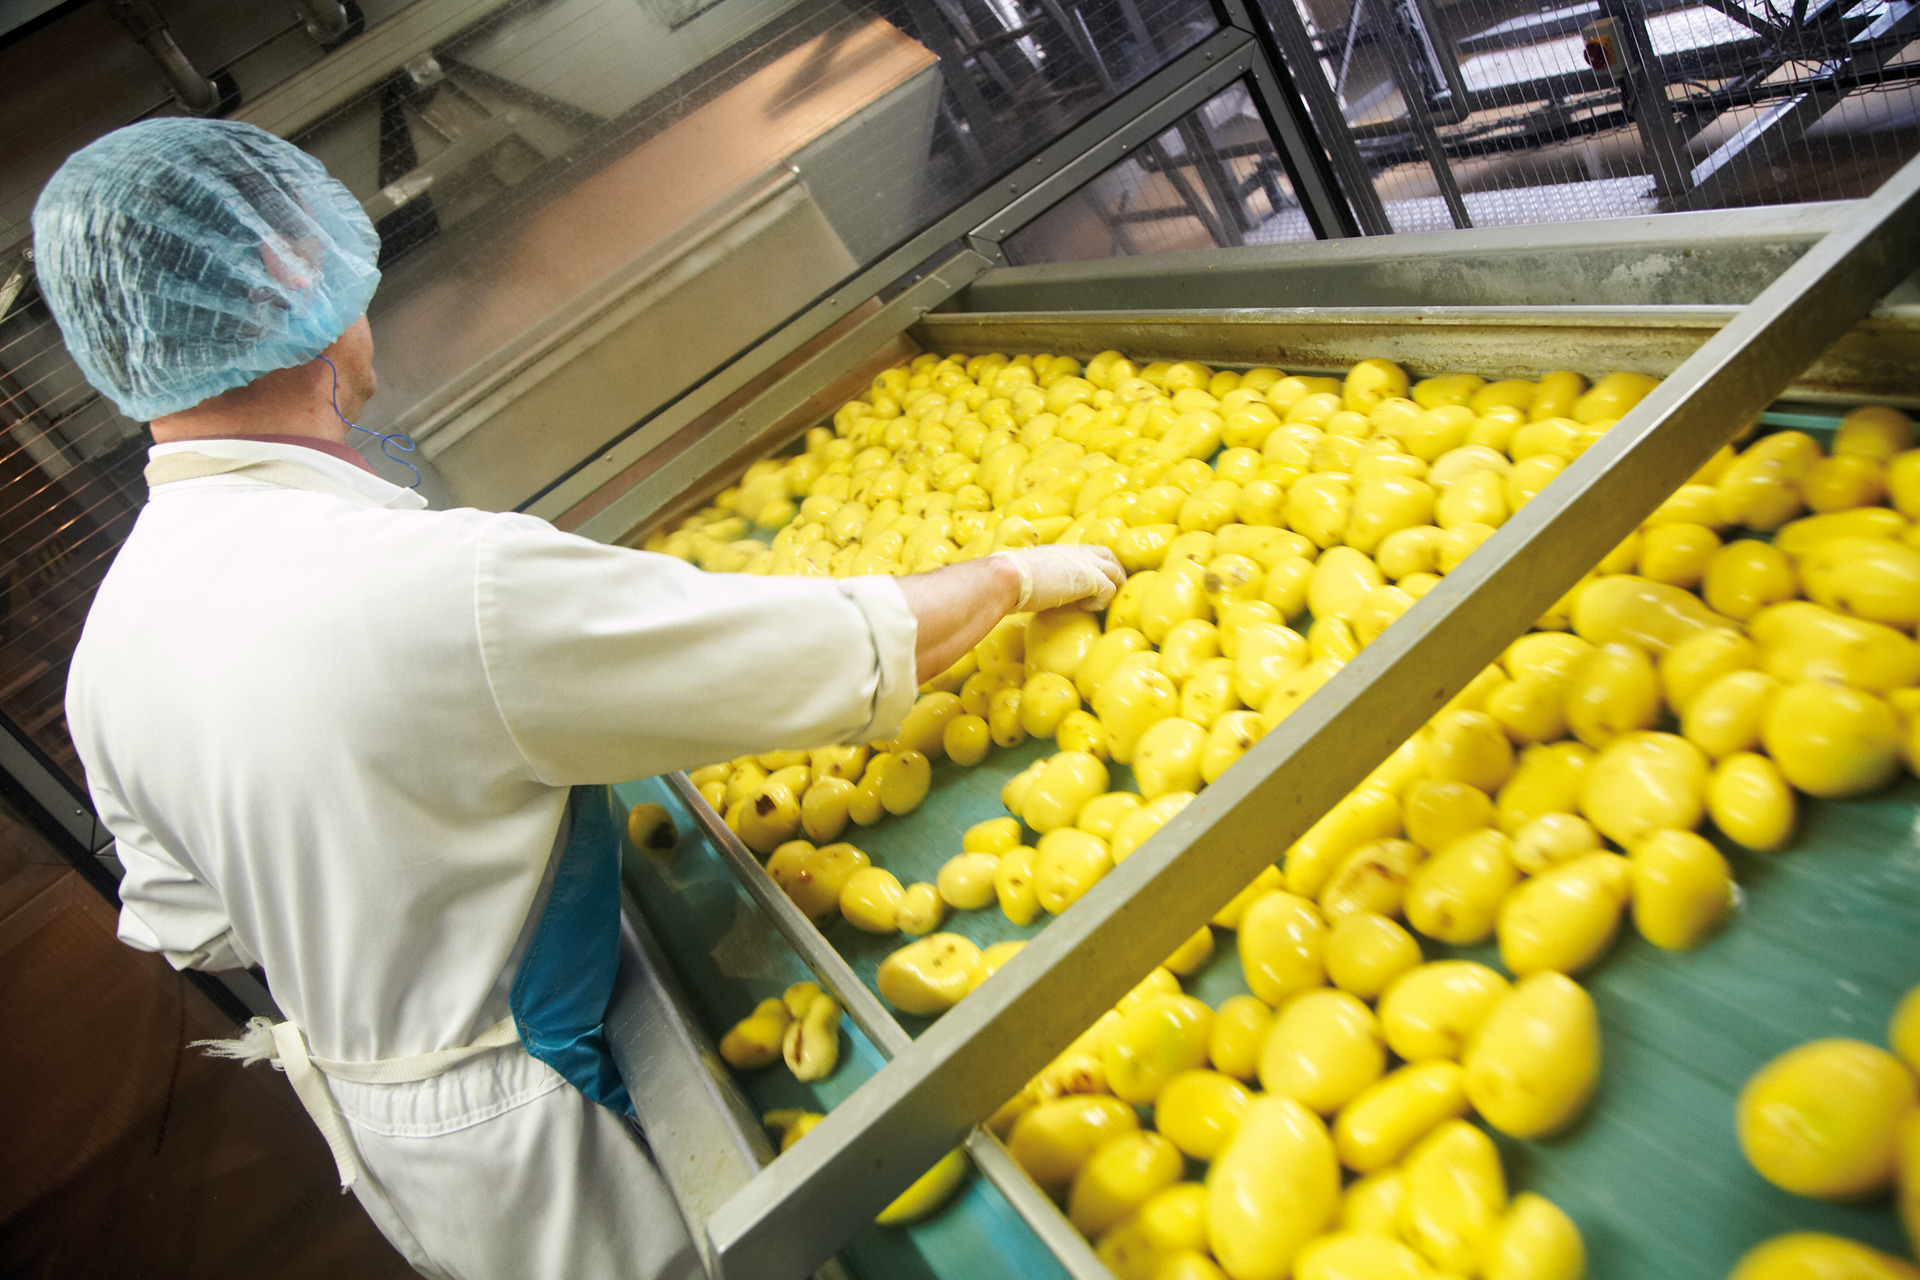
\includegraphics[width=0.95\textwidth]{images/motivacion/quality_control.png}
                    \end{column}
    \end{columns}
\end{frame}

\section{Conceptos previos}
\begin{frame}{Conceptos Previos - Redes Neuronales Convolucionales (CNNs)}
    \begin{columns}
        \begin{column}{0.5\textwidth}
            \begin{itemize}
                \item Las CNNs son un tipo de red neuronal profunda diseñadas para procesar datos con una estructura de cuadrícula, como imágenes.
                \item El objetivo es localizar dentro de una imagen objetos y clasificarlos, detectando defectos o características específicas.
                \item Utilizan capas convolucionales para extraer características jerárquicas.
                \item Existen dos tipos principales de CNNs, detectores de dos etapas como R-CNN y detectores de una etapa como YOLO.
                    
            \end{itemize}
        \end{column}
        \begin{column}{0.5\textwidth}
            \includegraphics[width=0.95\textwidth]{images/conceptos_previos/diagrama_de_Venn_inteligencia_artificial.png}
            \includegraphics[width=0.95\textwidth]{images/conceptos_previos/yolo.png}
        \end{column}
    \end{columns}
\end{frame}

\begin{frame}{Conceptos Previos - Hardware NVIDIA Jetson}

    \begin{columns}
        \begin{column}{0.5\textwidth}
            \begin{itemize}
                \item Arquitecturas de dominio específico y uso del paradigma \textit{manycore} para acelerar el procesamiento de IA.
                \item NVIDIA Jetson: CPU y GPU en un chip para eficiencia energética y procesamiento paralelo.
                \item TensorRT: optimiza modelos para inferencia en hardware NVIDIA. cuDNN y cuBLAS aceleran operaciones de redes neuronales y álgebra lineal.          
            \end{itemize}
        \end{column}
        \begin{column}{0.5\textwidth}
            %\includegraphics[width=0.95\textwidth]{images/motivacion/jetson_family.png}
            \includegraphics[width=1\textwidth]{images/conceptos_previos/TensorRT_optimizaciones.png}
            \includegraphics[width=1\textwidth]{images/conceptos_previos/TensorRT_pipeline.png}
        \end{column}
    \end{columns}
\end{frame}

\begin{frame}{Conceptos Previos - Seguimiento de objetos (MOT)}
    % \begin{columns}
    %     \begin{column}{0.4\textwidth}
    %         \begin{itemize}
    %             \item El seguimiento de objetos es una técnica que permite identificar y seguir la trayectoria de un objeto a lo largo del tiempo en una secuencia de imágenes.
    %             \item Combina técnicas de detección y análisis de movimiento para mantener el seguimiento preciso incluso en condiciones cambiantes.
    %             \item BYTETrack es un algoritmo de seguimiento de objetos que utiliza características visuales y de movimiento para mantener el seguimiento de múltiples objetos en movimiento.
    %         \end{itemize}
    %     \end{column}
    %     \begin{column}{0.7\textwidth}
    %         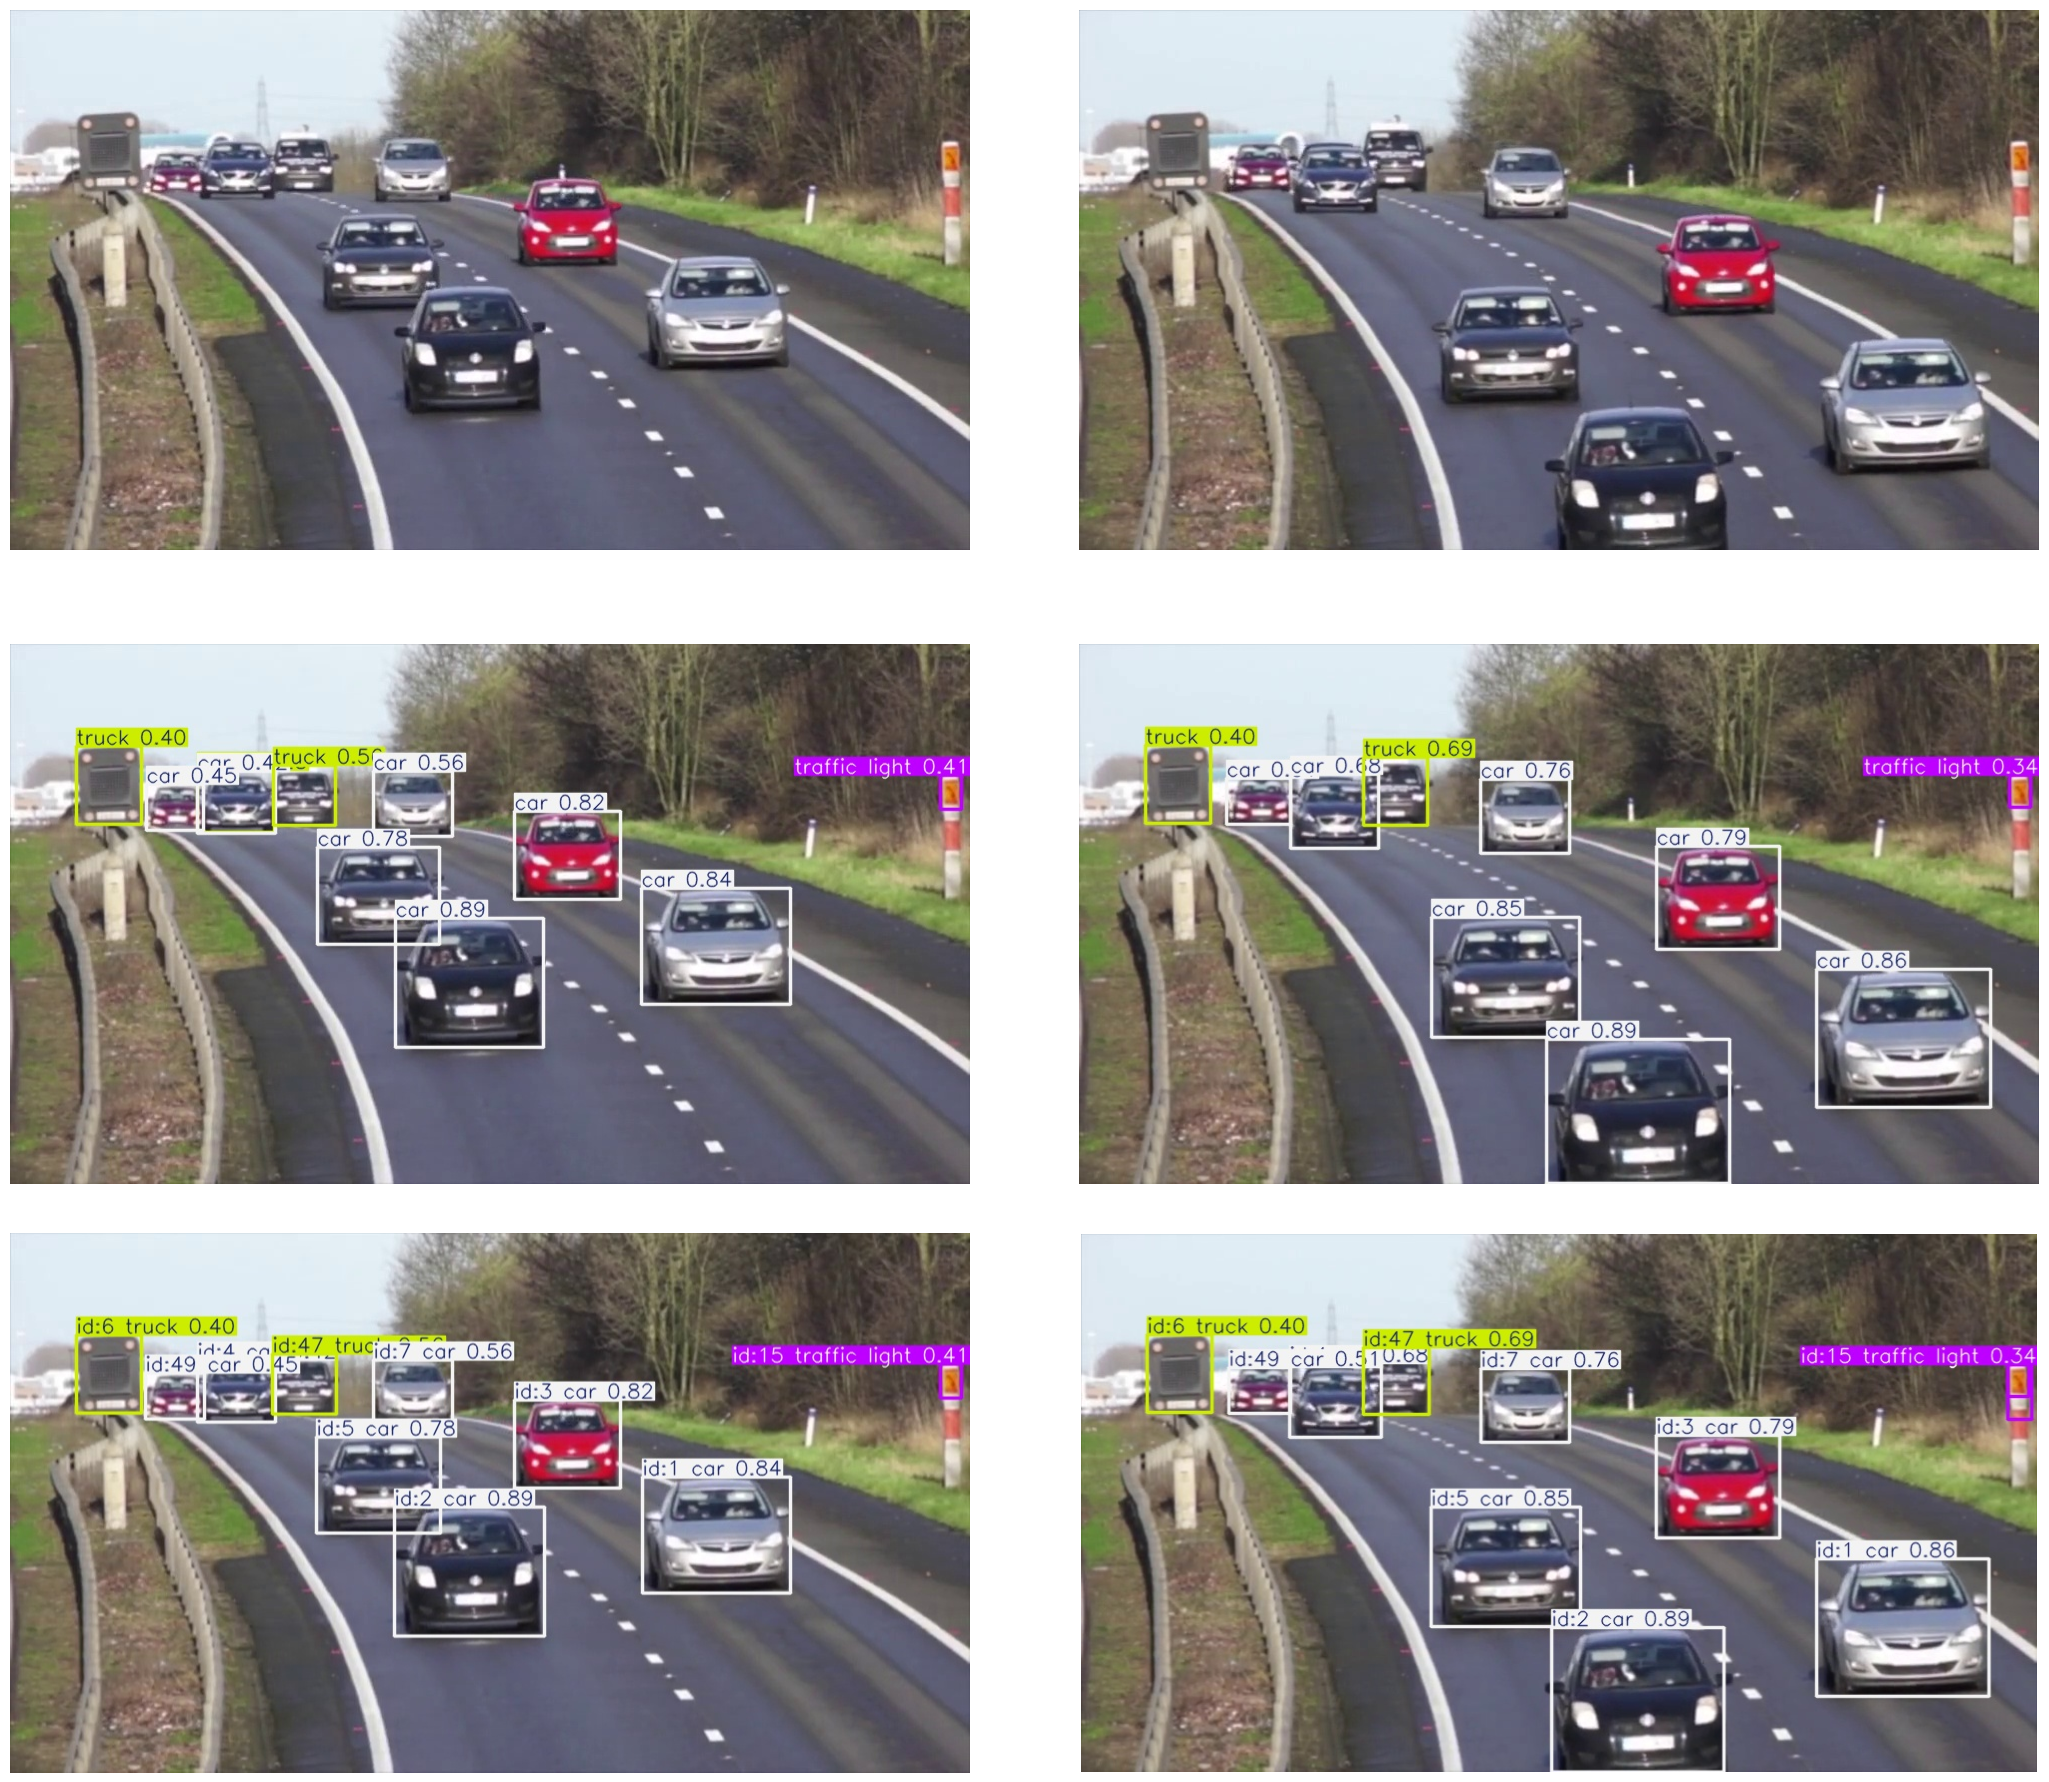
\includegraphics[width=1\textwidth]{images/conceptos_previos/tracking.png}
    %     \end{column}
    % \end{columns}
    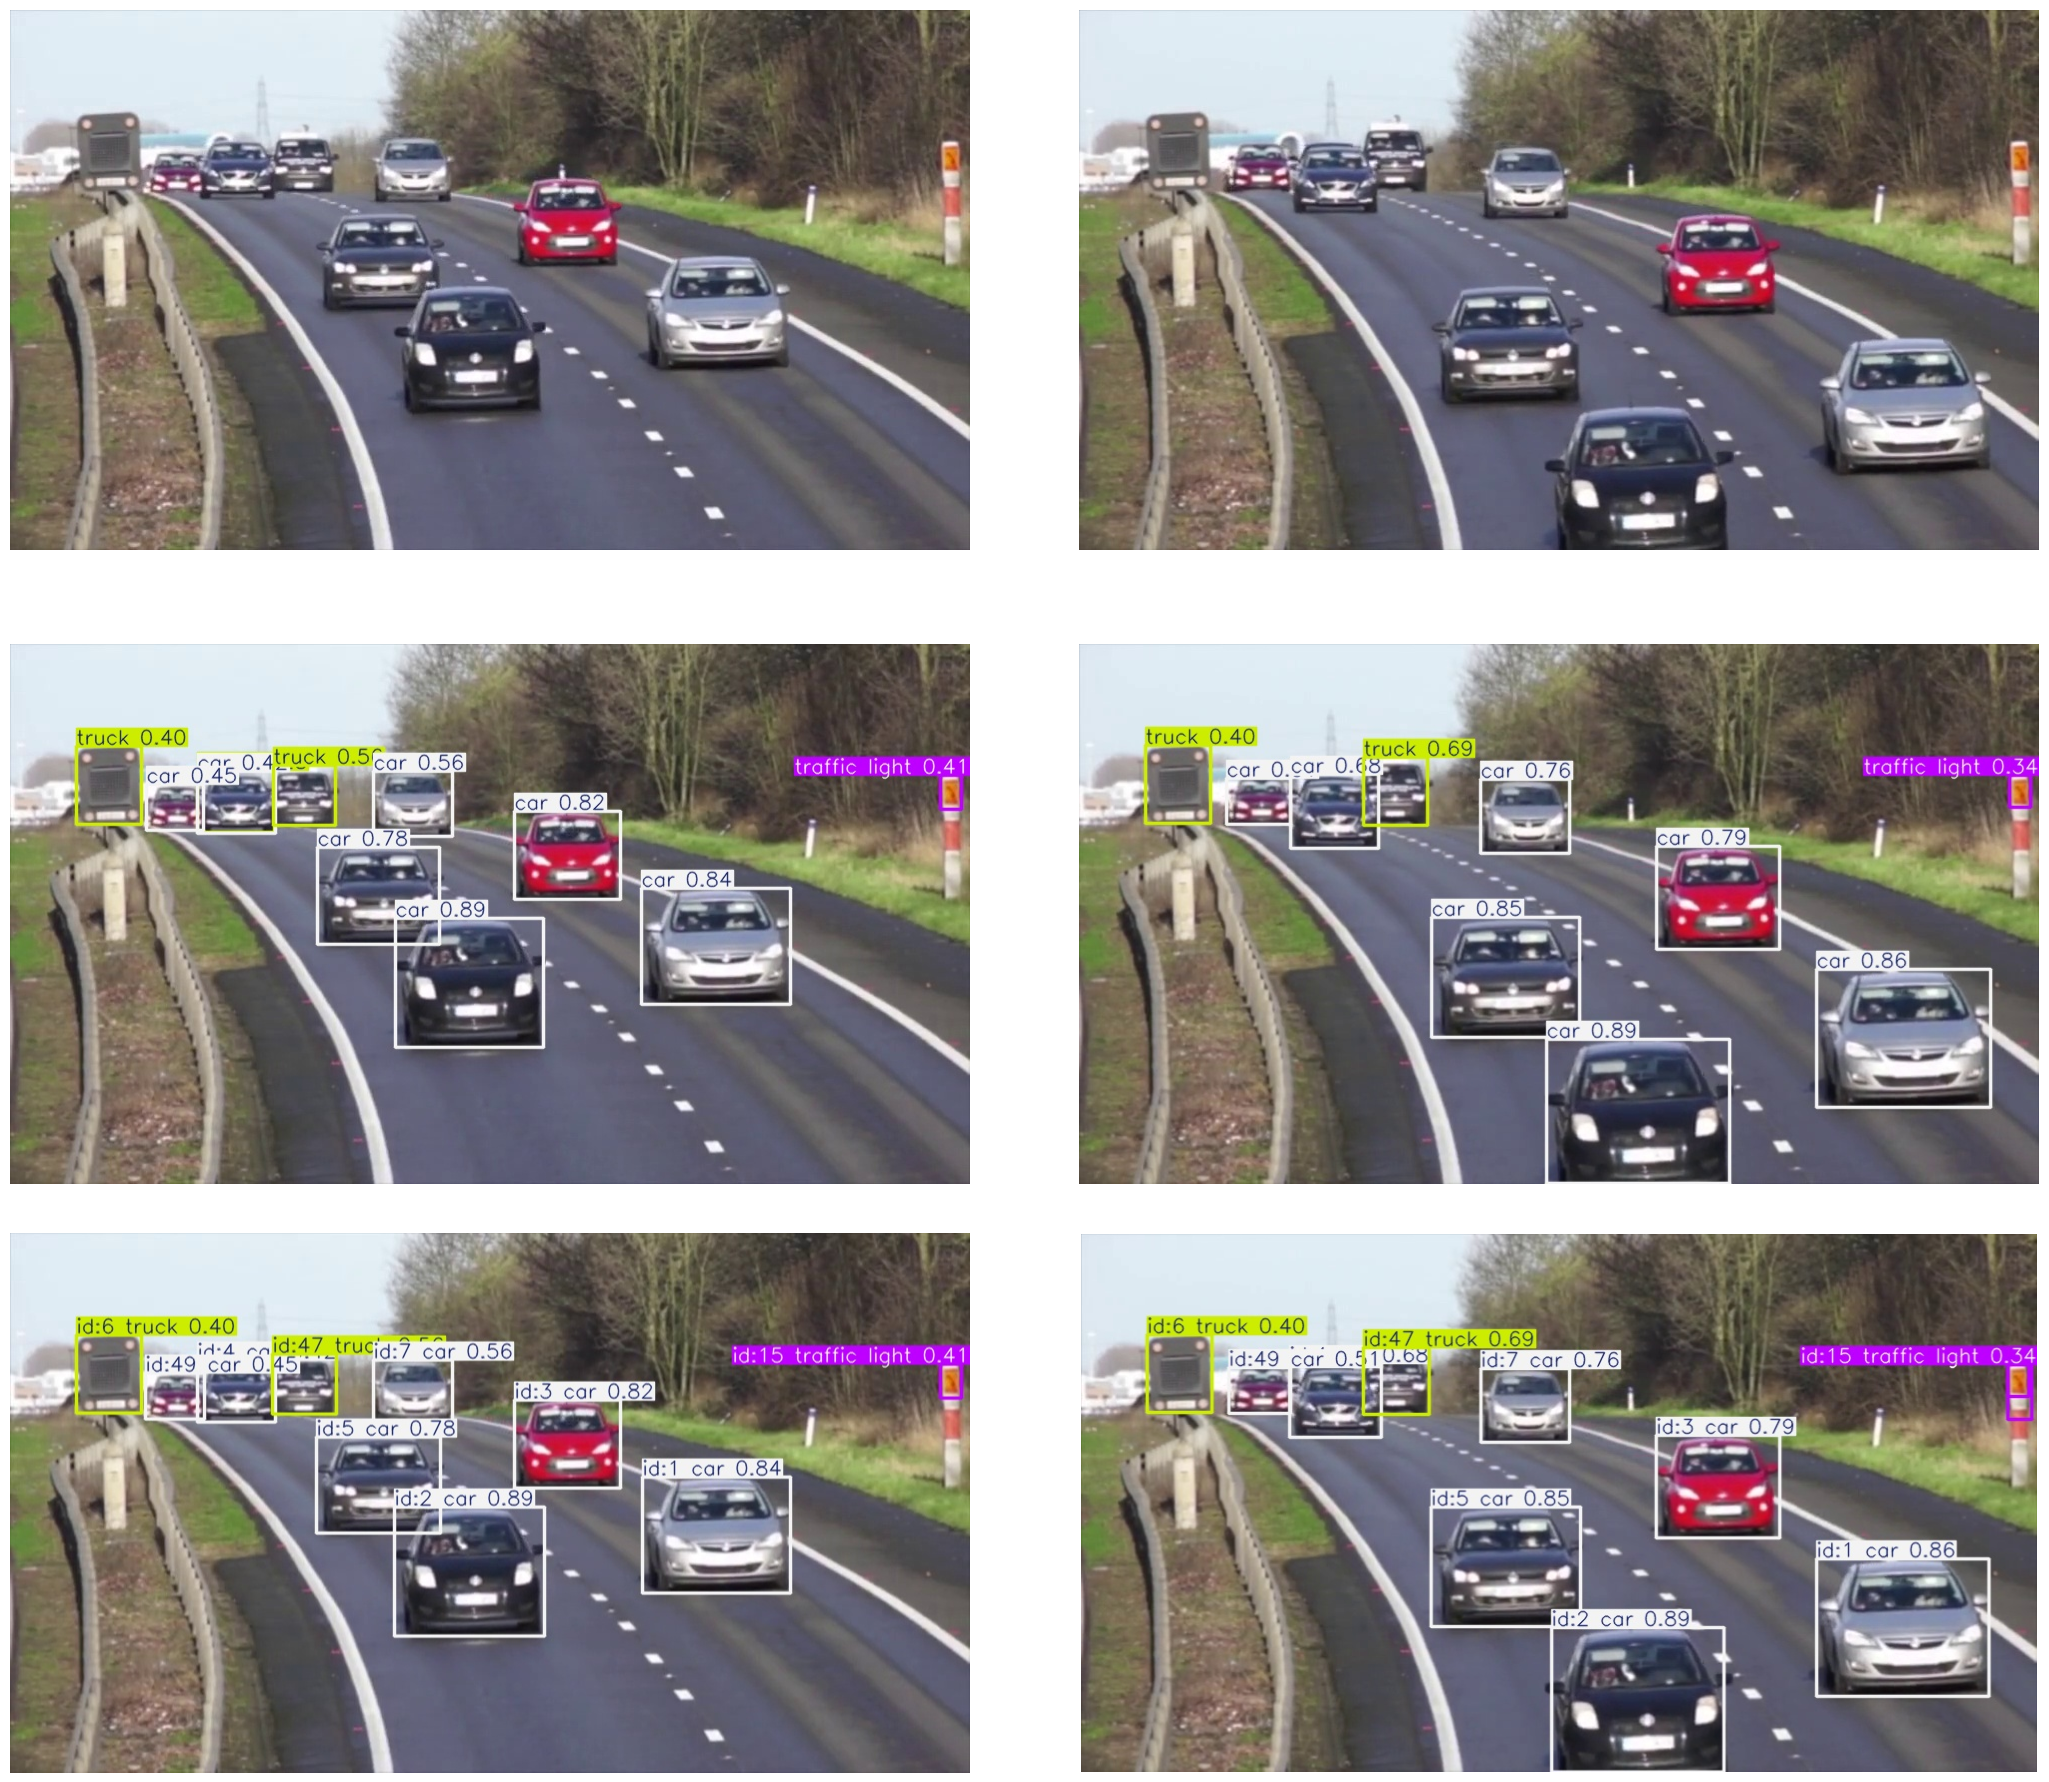
\includegraphics[width=0.9\textwidth]{images/conceptos_previos/tracking.png}


\end{frame}

\section{Análisis del problema}
\begin{frame}{Análisis del problema}
    Este trabajo se centra en desarrollar un sistema de visión artificial capaz de detectar defectos y realizar el seguimiento en tiempo real de múltiples objetos en movimiento, usando hardware NVIDIA Jetson por su eficiencia energética. Dado que no se dispone de un entorno industrial real, se utilizó un entorno simulado con canicas de distintos colores y defectos para representar objetos en una línea de producción. Este enfoque permite evaluar el rendimiento del sistema de forma controlada, sentando las bases para su futura aplicación en escenarios industriales reales.
\end{frame}

\section{Objetivos}
\begin{frame}{Objetivos}
    \begin{itemize}
        \item Estudiar el estado del arte en CNNs, aceleradores y optimización.
        \item Crear un conjunto de datos para entrenamiento y evaluación.
        \item Entrenar y validar modelos CNN para detección de defectos en tiempo real.
        \item Implementar un sistema de visión artificial integrado con hardware NVIDIA.
        \item Analizar y optimizar cuellos de botella para mejorar rendimiento y eficiencia.
        \item Evaluar el sistema con métricas de precisión, latencia y consumo.
        \item Realizar un análisis comparativo para encontrar la configuración óptima.
    \end{itemize}
\end{frame}

\section{Propuesta de solución}
\begin{frame}{Propuesta de solución}
\end{frame}

\section{Desarrollo de la solución}

\begin{frame}{Desarrollo de la solución - Entrenamiento y validación de modelos}
\end{frame}

\begin{frame}{Desarrollo de la solución - Optimización de los modelos para hardware NVIDIA}
\end{frame}

\begin{frame}{Desarrollo de la solución - Descripción de las etapas del sistema}
    \begin{itemize}
        \item Captura de imágenes.
        \item Preprocesamiento.
        \item Inferencia con CNNs.
        \item Postprocesamiento y visualización.
    \end{itemize}
\end{frame}

\begin{frame}{Desarrollo de la solución - Segmentación de las etapas}
\end{frame}

\section{Demo del sistema}
\begin{frame}{Demo del sistema}
\end{frame}

\section{Resultados}
\begin{frame}{Resultados}
\end{frame}

\section{Conclusiones}
\begin{frame}{Conclusiones}
    \begin{itemize}
        \item Se ha desarrollado un sistema de detección de defectos en objetos en movimiento.
        \item Se ha optimizado el rendimiento para hardware NVIDIA.
        \item Los resultados muestran una mejora en precisión y eficiencia.
    \end{itemize}
\end{frame}

\end{document}








% % Primera sección
% \section{A}

% \begin{frame}{¿Qué es LaTeX Beamer?}
%     \begin{itemize}
%         \item Beamer es una clase de LaTeX para crear presentaciones
%         \item Permite crear diapositivas profesionales
%         \item Muy utilizado en el ámbito académico
%         \item Soporte completo para matemáticas: $E = mc^2$
%     \end{itemize}
% \end{frame}

% % Segunda sección
% \section{Características principales}

% \begin{frame}{Ventajas de Beamer}
%     \begin{enumerate}
%         \item \textbf{Control total} sobre el formato
%         \item \textbf{Consistencia} en el diseño
%         \item \textbf{Ecuaciones} matemáticas perfectas
%         \item \textbf{Referencias} automáticas
%     \end{enumerate}
    
%     \vspace{1cm}
    
%     \begin{block}{Ejemplo de bloque}
%         Los bloques son útiles para destacar información importante.
%     \end{block}
% \end{frame}

% \begin{frame}{Ejemplo con columnas}
%     \begin{columns}
%         \begin{column}{0.5\textwidth}
%             \textbf{Columna izquierda:}
%             \begin{itemize}
%                 \item Punto 1
%                 \item Punto 2
%                 \item Punto 3
%             \end{itemize}
%         \end{column}
        
%         \begin{column}{0.5\textwidth}
%             \textbf{Columna derecha:}
%             \begin{itemize}
%                 \item Otro punto 1
%                 \item Otro punto 2
%                 \item Otro punto 3
%             \end{itemize}
%         \end{column}
%     \end{columns}
% \end{frame}

% % Tercera sección
% \section{Conclusiones}

% \begin{frame}{Conclusiones}
%     \begin{alertblock}{Importante}
%         Beamer es una excelente herramienta para presentaciones académicas.
%     \end{alertblock}
    
%     \vspace{0.5cm}
    
%     \begin{itemize}
%         \item Fácil de aprender
%         \item Resultados profesionales
%         \item Altamente personalizable
%     \end{itemize}
    
%     \vspace{1cm}
    
%     \centering
%     \Large ¡Gracias por su atención!
% \end{frame}

% \end{document}